
\documentclass[xcolor=dvipsnames, compress, t]{beamer}

\usetheme{CambridgeUS}
\usepackage[english]{babel}
\usepackage{color}
\usepackage{graphics}
\usepackage{graphicx}
\usepackage{stmaryrd}
\usepackage{etoolbox}
\usepackage{multicol}
\usepackage{tikz}
\usetikzlibrary{positioning,shapes.geometric, arrows}
\usepackage{booktabs}

\usepackage{dsfont}
\usepackage{etoolbox}
\usepackage{accents}
\usepackage{sgame}
\usepackage{epstopdf}
\usepackage{wrapfig}
\usepackage{tabto}

\setbeamertemplate{theorems}[numbered]
\undef{\lemma}
\newtheorem{lemma}{\translate{Lemma}} %gives own numbered lemmas
\newtheorem{prop}{Proposition}
\newtheorem{defin}{Definition}
\newenvironment{sketch}[1][Sketch of Proof.]{ \begin{trivlist} \item[\hskip \labelsep {\bfseries #1}]}{\end{trivlist}}

%colors

\definecolor{NIUred}{RGB}{200,16,46 } 
\definecolor{NIUblack}{RGB}{0,0,0}
\definecolor{NIUpantone}{RGB}{165,167,168}

\setbeamercolor{palette primary}{bg=NIUblack,fg=white}
\setbeamercolor{palette secondary}{bg=NIUpantone,fg=white}
\setbeamercolor{palette tertiary}{bg=NIUred,fg=white}
\setbeamercolor{palette quaternary}{bg=NIUred,fg=white}
\setbeamercolor{structure}{fg=NIUred} % itemize, enumerate, etc
\setbeamercolor{section in toc}{fg=NIUred} % TOC sections
%\setbeamercolor{subsection in head/foot}{bg=NIUpantone,fg=white}
%%Special Commands
\newcommand\munderbar[1]{%
	\underaccent{\bar}{#1}}

\newcommand{\der}{\mathrm{d}}
\newcommand{\e}{\mathrm{e}}

\newcommand{\vs}{\vspace{\baselineskip}}
\newcommand{\vf}{\vspace{5pt}}
\newcommand{\draw}{{\color{Plum} \bf Drawing.}} 
%use this if there is a drawing that you can't include
\newcommand{\wts}[1]{{\color{Orchid} \textbf{\underline{WTS}:}  #1}} 
%use this for what to show!

\setbeamertemplate{navigation symbols}{} 
\setbeamertemplate{enumerate items}[default]

%%Don't change things above this%%

%%%%%%%%%%%%%%%%%%


\title[ECON 592: ECONference Presentation]{Measuring the Fed-Information Effect}
\author{Ethan Rahman}
\institute[NIU]{\vspace{-10pt} \large Northern Illinois University}
\date{April 13, 2022}

\renewcommand{\thedefin}{4.\Alph{defin}} %ended on 4.C
\setcounter{defin}{3}

\renewcommand{\thetheorem}{4.\arabic{theorem}} %ended on 4.2
\setcounter{theorem}{2}

\renewcommand{\thelemma}{4.\roman{lemma}}
\setcounter{lemma}{0}

\usepackage[style=apa]{biblatex}
\addbibresource{refs.bib}
\renewcommand*{\bibfont}{\scriptsize}

\setbeamerfont{caption}{size=\tiny}

\begin{document}
	\begin{frame}
		\titlepage
	\end{frame}
	\begin{frame}{Introduction}
		\begin{itemize}
			\item Monetary Policy 
			\begin{itemize}
				\item<2-> Crucial for stabilizing the business cycle
				\item<3-> Maximum employment and stable prices
				\item<4-> Faster and more responsive than fiscal policy
			\end{itemize}
		\end{itemize}
		\begin{figure}
			\includegraphics<5->[width=.66\textwidth]{charts/ffrRgdp.png}
			\visible<5->{\caption{\cite{beaRGDP} \cite{bogFFER}}}
		\end{figure}
	\end{frame}
	\begin{frame}{Related Literature}
		\begin{itemize}
			\item \citeauthor{Romer2004} (\citeyear{Romer2004}) 
			\begin{itemize}
				\item<2-> Federal Reserve's internal "Greenbook forecasts"
				\item<2-> Regress FFR changes on forecasts
				\item<2-> Use the residual as indicator
			\end{itemize}
			\item<3-> \citeauthor{Nakamura2018} (\citeyear{Nakamura2018})
			\begin{itemize}
				\item<4-> FFR Futures contract prices
				\item<4-> High frequency identification
				\item<4-> Unexpected rate changes are the indicator
			\end{itemize}
			\item<5-> \citeauthor{Bauer2020} (\citeyear{Bauer2020}) 
			\begin{itemize}
				\item<6-> Presents "Fed-information effect" 
				\item<6-> Implies Nakamura indicator has omitted variable bias
			\end{itemize}
		\end{itemize}
	\end{frame}
	\begin{frame}{Economic Theory}
		\begin{itemize}
			\item<2-> \[
			i_m = i_m^p(\text{PubInfo}_m) + X_m(\text{FedInfo}_m)^\prime \alpha + \epsilon_m 
			\]
			\begin{itemize}
				\item<2-> \(i_m^p\): Private sector forecast of \(i_m\)
				\item<2->\(X_m\): Vector of state variable forecasts
				\item<2-> \(\epsilon_m\): Exogenous monetary policy shock
			\end{itemize}
			\item<3-> Can use FFR futures prices to measure \(i_m^p\) (\cite{Gurkaynak2011}; \cite{Gertler2015}; \cite{Nakamura2018})
			\item<4-> 
				\begin{align*}
					i_m - i_m^p(\text{PubInfo}_m) &= X_m(\text{FedInfo}_m)^\prime \alpha + \epsilon_m \\
					FS_m &= X_m(\text{FedInfo}_m)^\prime \alpha + \epsilon_m 
				\end{align*}
			\(FS_m\): Change in FFR Futures price over a 30 minute window around FOMC announcement corresponding to meeting \(m\)
		\end{itemize}
	\end{frame}
	\begin{frame}{Economic Theory}
		\begin{itemize}
			\item<2-> The Fed-information effect: \(FS_m\) and \(X_m(\text{FedInfo}_m)\) could be correlated
			\item<3-> Suppose we have some variable \(y_m\)...
			\begin{align*}				
				y_m &= \beta_0 + \beta_1 \epsilon_m  + v \\
				y_m &= \beta_0 + \beta_1(FS_m - X_m(\text{FedInfo}_m)^\prime \alpha )  + v \\
				y_m &= \beta_0 + \beta_1FS_m - \beta_1 X_m(\text{FedInfo}_m)^\prime \alpha + v \\
				y_m &= \beta_0 + \beta_1FS_m + u \tag{4} \label{eq3} \\ 
				\mathrm{Cov}(FS_m, u) &\neq 0 
			\end{align*}
		\end{itemize}
	\end{frame}
	\begin{frame}{Data}
		\begin{itemize}
			\item<2-> For \(FS_m\), the data for \citeauthor{Nakamura2018} (\citeyear{Nakamura2018}) is publicly available.
			\item<3-> For \(X_m\), I use the Greenbook Forecasts
			\item<4-> Model very similar to \citeauthor{Romer2004} (\citeyear{Romer2004}):
			\begin{align*}
				FS_m =  \alpha &+ \sum_{i=0}^{2} \gamma_i \widetilde{\Delta y}_{mi} + \sum^2_{i=0} \lambda_i \left(\widetilde{\Delta y}_{mi}-\widetilde{\Delta y}_{m-1,i}\right)\\
				&+\sum^{2}_{i=0} \phi_i \tilde{\pi}_{mi} + \sum^2_{i=0} \theta_i \left(\tilde{ \pi}_{mi}-\tilde{ \pi}_{m-1,i}\right) + \rho \tilde{u}_{m0} + \epsilon_m
			\end{align*}
			\item<5-> Use \(\hat{\epsilon_m}\) as our new indicator
			\item<6-> For \(y_m\), I follow the methodology of \citeauthor{Bauer2020} (\citeauthor{Bauer2020}) and use the 24 hour change in the log of the S\&P500 stock market index. 
		\end{itemize}
	\end{frame}
	\begin{frame}{Data}
		\begin{figure}
			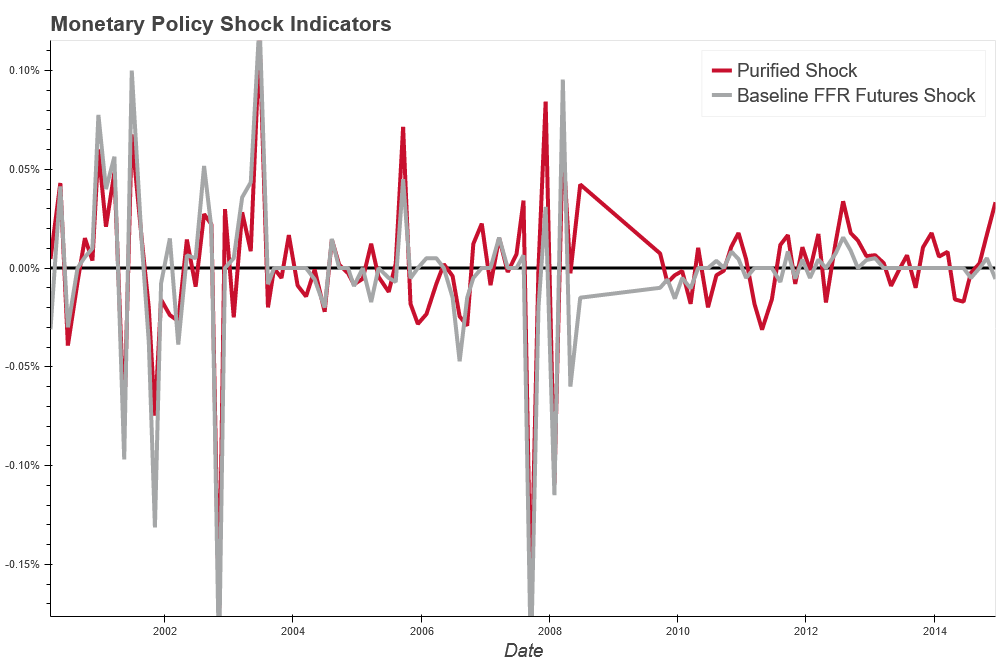
\includegraphics[width=.90\textwidth]{charts/pure_indicator.png}
		\end{figure}
	\end{frame}
	\begin{frame}{Empirical Analysis}
		\begin{itemize} 
			\item<2-> Model 1 (same as \cite{Bauer2020}):
				\[
					\Delta \log{(\text{S\&P500}_m)} = \beta_0 + \beta_1 FS_m + u 
				\]
			\item<3-> Model 2: 
				\[
					\Delta \log{(\text{S\&P500}_m)} = \delta_0 + \delta_1 \hat{\epsilon}_m + w
				\]
		\end{itemize}
	\end{frame}
	\begin{frame}{Empirical Analysis: Wu-Hausman Test}
		\begin{align*}
			\uncover<2->{H_0: &\delta_1 \text{ and } \beta_1 \text{ are consistent.}} \\
			\uncover<2->{H_a: &\delta_1 \text{ is consistent but } \beta_1 \text{ is inconsistent.}}
		\end{align*}
		\begin{align*}
			\uncover<3->{\text{Test statistic: } &H = \frac{(\hat{\delta}_1-\hat{\beta}_1^R)^2}{\mathrm{Var}(\hat{\delta}_1)-\mathrm{Var}(\hat{\beta}_1^R)} \sim \chi^2_1} \\
			\uncover<4->{&H = \frac{( -7.154+6.518)^2}{2.919^2- 2.601^2} = .2304}
		\end{align*}
	\end{frame}
	\begin{frame}{References}
		\bibbysection
	\end{frame}
\end{document}